\documentclass[tikz,border=5pt]{standalone}
\usepackage{amsmath,amssymb}
\usetikzlibrary{arrows.meta,positioning,calc}
\begin{document}
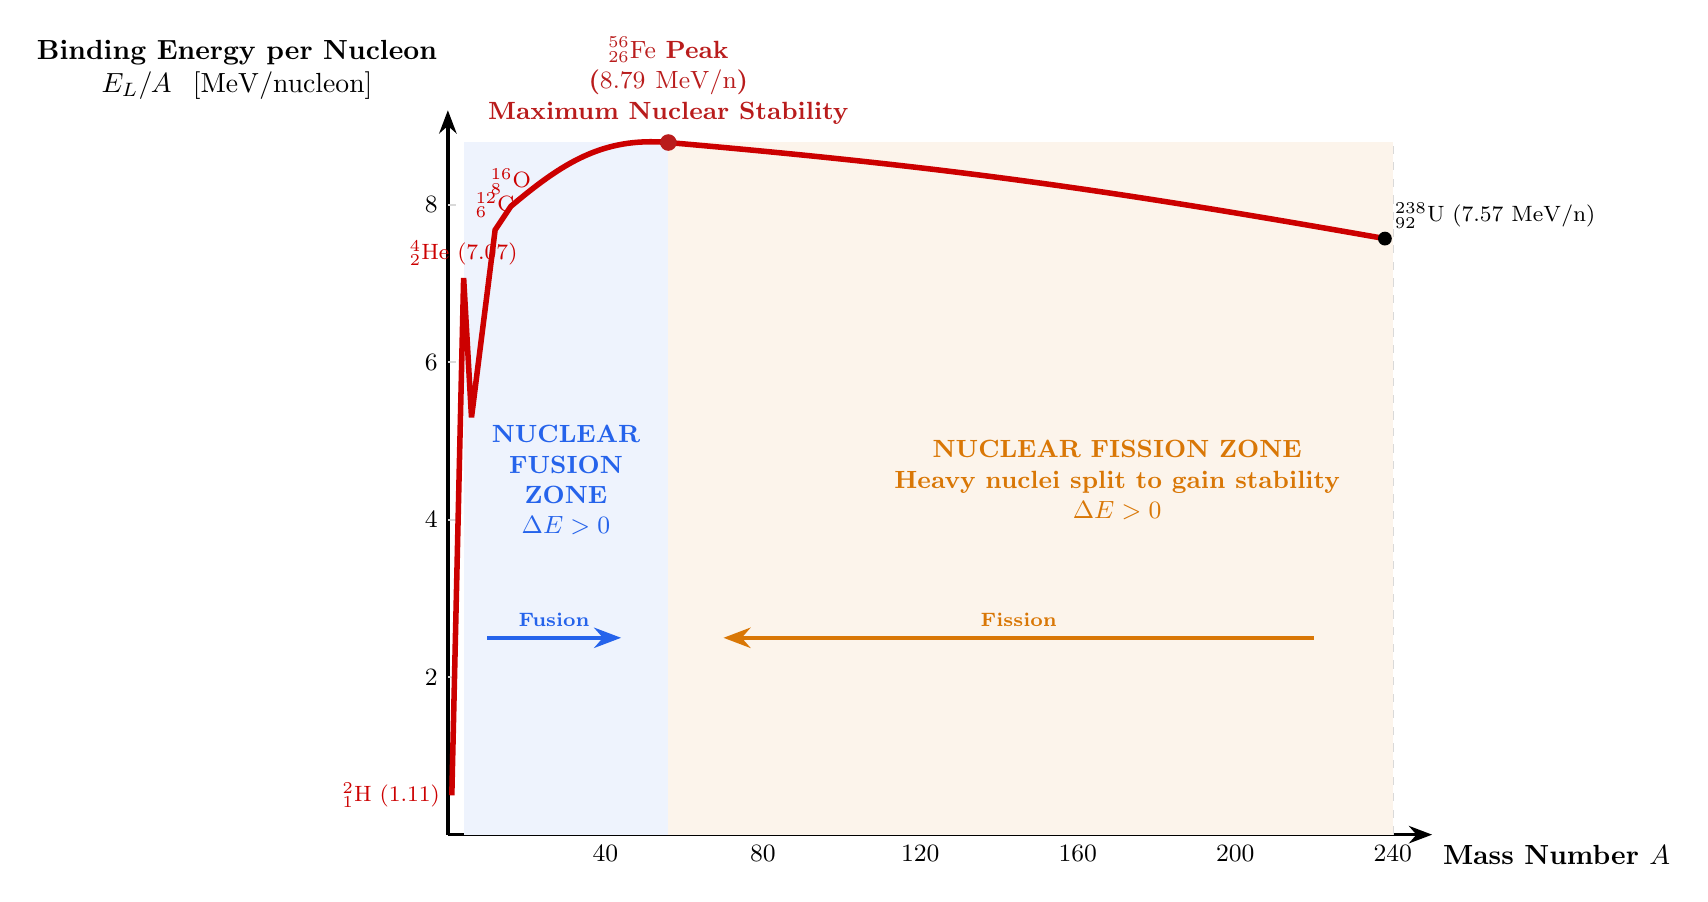
\begin{tikzpicture}[>=Stealth, font=\sffamily, thick]
  \definecolor{fe56}{HTML}{B91C1C}
  \definecolor{fusioncolor}{HTML}{2563EB}
  \definecolor{fissioncolor}{HTML}{D97706}

  % Axes
  \draw[->, line width=1.2pt] (0,0) -- (12.5,0) node[below right, font=\bfseries] {Mass Number $A$};
  \draw[->, line width=1.2pt] (0,0) -- (0,9.2) node[above left, font=\bfseries, align=center] {Binding Energy per Nucleon\\$E_L / A\ \ [\mathrm{MeV/nucleon}]$};

  % Grid & Ticks
  \foreach \y in {2,4,6,8} {
    \draw[gray!30, dashed] (0,\y) -- (12,\y);
    \node[left, font=\small] at (0,\y) {\y};
  }
  \foreach \x/\label in {2/40, 4/80, 6/120, 8/160, 10/200, 12/240} {
    \draw[gray!30, dashed] (\x,0) -- (\x,8.8);
    \node[below, font=\small] at (\x,0) {\label};
  }

  % Shaded regimes
  \fill[fusioncolor!8] (0.2,0) rectangle (2.8,8.8);
  \node[text=fusioncolor, font=\bfseries\small, align=center] at (1.5,4.5) {NUCLEAR\\FUSION\\ZONE\\$\Delta E > 0$};

  \fill[fissioncolor!8] (2.8,0) rectangle (12,8.8);
  \node[text=fissioncolor, font=\bfseries\small, align=center] at (8.5,4.5) {NUCLEAR FISSION ZONE\\Heavy nuclei split to gain stability\\$\Delta E > 0$};

  % Aston Curve Plot
  \draw[line width=2pt, red!80!black]
    (0.05, 0.5) node[left, font=\footnotesize] {$^2_1\mathrm{H}$ (1.11)}
    -- (0.2, 7.07) node[above, font=\footnotesize] {$^4_2\mathrm{He}$ (7.07)}
    -- (0.3, 5.3)
    -- (0.6, 7.68) node[above, font=\footnotesize] {$^{12}_6\mathrm{C}$}
    -- (0.8, 7.98) node[above, font=\footnotesize] {$^{16}_8\mathrm{O}$}
    to[out=40, in=175] (2.8, 8.79) % Peak Fe-56
    to[out=-5, in=170] (11.9, 7.57); % U-238

  % Peak Fe-56
  \fill[fe56] (2.8, 8.79) circle (3pt);
  \node[above=3pt, text=fe56, font=\bfseries\small, align=center] at (2.8, 8.79) {$^{56}_{26}\mathrm{Fe}$ Peak\\($8.79\ \mathrm{MeV/n}$)\\Maximum Nuclear Stability};

  % U-238
  \fill[black] (11.9, 7.57) circle (2.5pt);
  \node[above right, font=\footnotesize] at (11.9, 7.57) {$^{238}_{92}\mathrm{U}$ ($7.57\ \mathrm{MeV/n}$)};

  % Arrows indicating direction of exothermic energy release
  \draw[->, line width=1.5pt, fusioncolor] (0.5, 2.5) -- (2.2, 2.5) node[midway, above, font=\scriptsize\bfseries] {Fusion};
  \draw[<-, line width=1.5pt, fissioncolor] (3.5, 2.5) -- (11.0, 2.5) node[midway, above, font=\scriptsize\bfseries] {Fission};
\end{tikzpicture}
\end{document}
